
%%% Local Variables:
%%% mode: latex
%%% TeX-master: t
%%% End:

\chapter{盐田、大鹏中观交通模型建设}
延续深圳市交通仿真系统(二期)中观模型的建模思路和技术要求,采用德
国 PTV 公司 VISUM 软件作为建模工具,从模型数据准备开始,一直到现状模
型参数校核,重新搭建盐田、大鹏中观交通模型,包括现状年模型和规划年模型。
其中, 采用的全部现状数据都为 2018 年最新数据。

\section{盐田、大鹏中观交通模型路网总体设置}
VISUM 构建交通模型的总体设置包括交通系统的设置和道路等级的设置两
部分。中观交通模型的基本设置与宏观交通模型基本保持一致。

\subsection{交通系统}
相较于宏观交通模型,中观交通模型所涉及的交通系统仅包含私人小汽车出
行方式中的客车、货车和出租车,且在分配时将客车与出租车合并进行分配。

\renewcommand{\arraystretch}{0.8}
\begin{longtable}[c] {|C{0.1\textwidth}|C{0.1\textwidth}|C{0.1\textwidth}|
C{0.1\textwidth}|C{0.1\textwidth}|C{0.1\textwidth}|C{0.1\textwidth}|}
  \caption{交通系统集说明表\label{tbl:交通系统集说明表}}
  \hline
  \multicolumn{3}{|c|}{\bfseries 交通系统(Tsys)} & \multicolumn{2}{c|}{\bfseries 出行方式(Mode)} &
 \multicolumn{2}{c|}{\bfseries 需求组成(Dseg)} \\\hline

\multicolumn{1}{|c|}{编码} & \multicolumn{1}{c|}{名称} & \multicolumn{1}{c|}{类型}& 
\multicolumn{1}{c|}{编码} & \multicolumn{1}{c|}{名称} & 
\multicolumn{1}{c|}{编码} & \multicolumn{1}{c|}{名称} \\
\multicolumn{1}{|c|}{(Code)} & \multicolumn{1}{c|}{(Name)} & \multicolumn{1}{c|}{(Type)} & 
\multicolumn{1}{c|}{(Code)} & \multicolumn{1}{c|}{(Name)} & 
\multicolumn{1}{c|}{(Code)} & \multicolumn{1}{c|}{(Name)} \\\hline
A & 客车 & PrT & A & 客车 & A & 客车 \\\hline
GV & 货车 & PrT & GV & 货车 & GV & 货车 \\\hline
T & 出租车 & PrT & T & 出租车 & T & 出租车 \\\hline
\end{longtable}

\subsection{道路类型}
中观交通模型主要沿用宏观交通模型的方法进行分类,并局部增加完善两类
方法,辅道单向一车道、辅道单向两车道。道路类型代码表如表\ref{tbl:模型中道路类型编码表}所示。

\clearpage

\renewcommand{\arraystretch}{0.8}
\begin{longtable}[c] {|C{0.05\textwidth}|B{0.22\textwidth}|B{0.22\textwidth}|C{0.08\textwidth}|
C{0.1\textwidth}|C{0.15\textwidth}|}
  \caption{模型中道路类型编码表\label{tbl:模型中道路类型编码表}}
  \hline
  \multicolumn{1}{|c|}{\bfseries 编号} & \multicolumn{1}{c|}{\bfseries 名称} &  
\multicolumn{1}{c|}{\bfseries 交通系统} & \multicolumn{1}{c|}{\bfseries 车道数} &
\multicolumn{1}{c|}{\bfseries 通行能力} & \multicolumn{1}{c|}{\bfseries 自由流速度} \\\hline

0 & 施工封闭段 & B & 0 & 0 & 20 \\\hline
1 & 单行线 & B & 0 & 0 & 0 \\\hline
2 & 规划路 & B & 0 & 0 & 0 \\\hline
5 & 高速公路八车道 & A,GV,MiniB,T & 4 & 8800 & 120 \\\hline
6 & 高速公路六车道 & A,GV,MiniB,T & 3 & 6600 & 120 \\\hline
7 & 高速公路四车道 & A,GV,MiniB,T & 2 & 4400 & 120 \\\hline
10 & 一级公路八车道 & A,B,GV,MiniB,T & 4 & 5600 & 80 \\\hline
11 &  一级公路六车道 & A,B,GV,MiniB,T & 3 & 4200 & 80 \\\hline
12 &  一级公路四车道 & A,B,GV,MiniB,T & 2 & 2800 & 80 \\\hline
16 &  二级及以下公路四车道 & A,B,GV,MiniB,T & 2 & 1800 & 50 \\\hline
17 &  二级及以下公路两车道 & A,B,GV,MiniB,T & 1 & 900 & 45 \\\hline
25 &  快速路八车道 & A,B,MiniB,T & 4 & 6000 & 80 \\\hline
26 &  快速路六车道 & A,B,MiniB,T & 3 & 4500 & 80 \\\hline
27 &  快速路四车道 & A,B,MiniB,T & 2 & 3000 & 80 \\\hline
30 &  主干道分隔八车道 & A,B,GV,MiniB,T & 4 & 3931 & 60 \\\hline
31 &  主干道分隔六车道 & A,B,GV,MiniB,T & 3 & 2948 & 55 \\\hline
32 &  主干道分隔四车道 & A,B,GV,MiniB,T & 2 & 1966 & 50 \\\hline
34 &  主干道禁货分隔八车道 & A,B,MiniB,T & 4 & 3931 & 6\\\hline
35 &  主干道禁货分隔六车道 & A,B,MiniB,T & 3 & 2948 & 5\\\hline
36 &  主干道禁货分隔四车道 & A,B,MiniB,T & 2 & 1966 & 5\\\hline
40 &  主干道划线八车道 & A,B,GV,MiniB,T & 4 & 3686 & 55\\\hline
41 &  主干道划线六车道 & A,B,GV,MiniB,T & 3 & 2765 & 55\\\hline
42 &  主干道划线四车道 & A,B,GV,MiniB,T & 2 & 1843 & 50\\\hline
44 &  主干道禁货划线八车道 & A,B,MiniB,T & 4 & 3686 & 5\\\hline
45 &  主干道禁货划线六车道 & A,B,MiniB,T & 3 & 2765 & 5\\\hline
46 &  主干道禁货划线四车道 & A,B,MiniB,T & 2 & 1843 & 5\\\hline
50 &  次干道分隔六车道 & A,B,GV,MiniB,T & 3 & 2458 & 45\\\hline
51 &  次干道分隔四车道 & A,B,GV,MiniB,T & 2 & 1638 & 45\\\hline
52 &  次干道分隔两车道 & A,B,GV,MiniB,T & 1 & 819 & 35 \\\hline
54 &  次干道禁货分隔六车道 & A,B,MiniB,T & 3 & 2458 & 4\\\hline
55 &  次干道禁货分隔四车道 & A,B,MiniB,T & 2 & 1638 & 4\\\hline
56 &  次干道禁货分隔两车道 & A,B,MiniB,T & 1 & 819 & 35\\\hline
60 &  次干道划线六车道 & A,B,GV,MiniB,T & 3 & 2294 & 40\\\hline
61 &  次干道划线四车道 & A,B,GV,MiniB,T & 2 & 1530 & 40\\\hline
62 &  次干道划线两车道 & A,B,GV,MiniB,T & 1 & 765 & 35 \\\hline
64 &  次干道禁货划线六车道 & A,B,MiniB,T & 3 & 2294 & 4\\\hline
65 &  次干道禁货划线四车道 & A,B,MiniB,T & 2 & 1530 & 4\\\hline
66 &  次干道禁货划线两车道 & A,B,MiniB,T & 1 & 765 & 35\\\hline
70 &  支路四车道 & A,B,GV,MiniB,T & 2 & 1248 & 35 \\\hline
71 &  支路两车道 & A,B,GV,MiniB,T & 1 & 624 & 30 \\\hline
72 &  支路两车道在建 & A,B,GV,MiniB,T & 1 & 300 & 20 \\\hline
74 &  支路禁货四车道 & A,B,MiniB,T & 2 & 1248 & 35 \\\hline
75 &  支路禁货两车道 & A,B,MiniB,T & 1 & 624 & 30 \\\hline
80 &  匝道单向两车道 & A,B,GV,MiniB,T & 2 & 2400 & 40 \\\hline
81 &  匝道单向一车道 & A,B,GV,MiniB,T & 1 & 1200 & 40 \\\hline
82 &  辅道单向二车道 & A,B,GV,MiniB,T & 2 & 1200 & 40 \\\hline
83 &  辅道单向一车道 & A,B,GV,MiniB,T & 1 & 600 & 40 \\\hline
85 &  隧道八车道 & A,B,GV,MiniB,T & 4 & 6000 & 80 \\\hline
86 &  隧道六车道 & A,B,GV,MiniB,T & 3 & 4500 & 80 \\\hline
87 &  隧道四车道 & A,B,GV,MiniB,T & 2 & 3000 & 80 \\\hline
\end{longtable}

\subsection{交叉口车道通行能力}
中观交通模型对交叉口的分析可以达到车道级别,这要求在模型中输入各种
类型的交叉口的车道数和渠化设计和信号灯设置等,软件按照 HCM2010 的方法
标定车道通行能力。参考香港 BDTM 模型设定,交叉口车道通行能力如下表所
示。如果进口道受到某些影响,例如车辆上下客,公交停靠,车辆交织等情况,
将根据实际情况对进口道饱和流率进行调整,实际符合实际情况。

\clearpage
\begin{table}[!ht]
\renewcommand{\arraystretch}{0.8} \centering
\caption[交叉口车道通行能力表]{交叉口车道通行能力表 \protect\footnotemark \label{tbl:交叉口车道通行能力表}}
\begin{tabular} {|C{0.3\textwidth}|C{0.15\textwidth}|C{0.15\textwidth}|C{0.15\textwidth}|}    
  \hline
  \multirow[c]{2}*{\bfseries 交叉口类型} & \multicolumn{3}{|c|}{\bfseries 每车道通行能力( pcu/h)}\\\cline{2-4} 
  & 左转 & 直行 & 右转\\\hline
信号控制交叉口 & 1650 & 2000 & 1850 \\\hline
让行交叉口--主要道路 & 1650 & 2000 & 800 \\\hline
让行交叉口--次要道路 & 1100 & 850 & 500 \\\hline
环形交叉口 & 1650 & 1650 & 1650 \\\hline
非信号控制交叉口 & 1100 & 1100 & 1100 \\\hline
\end{tabular}
\end{table}
\footnotetext{让行交叉口的主要道路的可穿越车头时距在能见度高时为 2.75 秒,能见度低时为 3.0 秒,
环岛通行内部通行能力为 2400pcu/hour,饱和车头时距为1.5 秒。}

\section{盐田、大鹏中观模型路网}
\subsection{中观区域现状路网截取}
为了保持路网的一致性,宏观交通模型也与中观交通模型一样包含次要支路,
因此,盐田、大鹏中观现状基础模型路网由深圳市宏观现状模型路网中截取,截
取方法如下:

\begin{nbeae}
\item 在宏观模型路网上,计算路段和转向的公交背景量,并将结果写入
Link 的 AddValue3 以及 Turn 的 AddValue3 属性(见图\ref{fig:chp05_公交背景量计算})。
在此采用了简化计算,我们假设所有公交线路在高峰小时的发车频率均为 6 分钟每班,则每条公交线路占用的
道路资源为 10 辆公交车辆/小时,按大车与标准车之间的折算系数 2 计算,每条
公交线路占用 20PCU 的路段资源。因此,路段的 AddValue3 属性等于路段通过
的公交线路数乘以 20,单位为 PCU。
\begin{figure}[!ht]
  \centering
  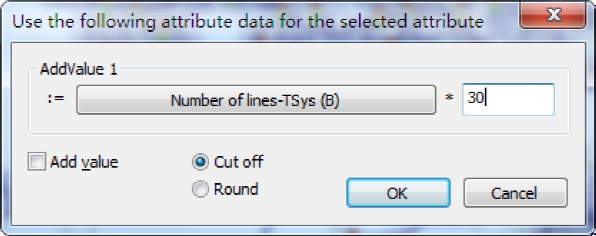
\includegraphics[width=0.7\textwidth]{chp05_公交背景量计算.jpg}
  \caption{公交背景量计算\label{fig:chp05_公交背景量计算} }
\end{figure}

\item 在宏观模型中加载盐田、大鹏中观基础模型范围的 SHP 文件(该 SHP
文件在 ArcGIS 中生成),如图\ref{fig:chp05_盐田大鹏宏观交通模型}所示。
\begin{figure}[!ht]
  \centering
  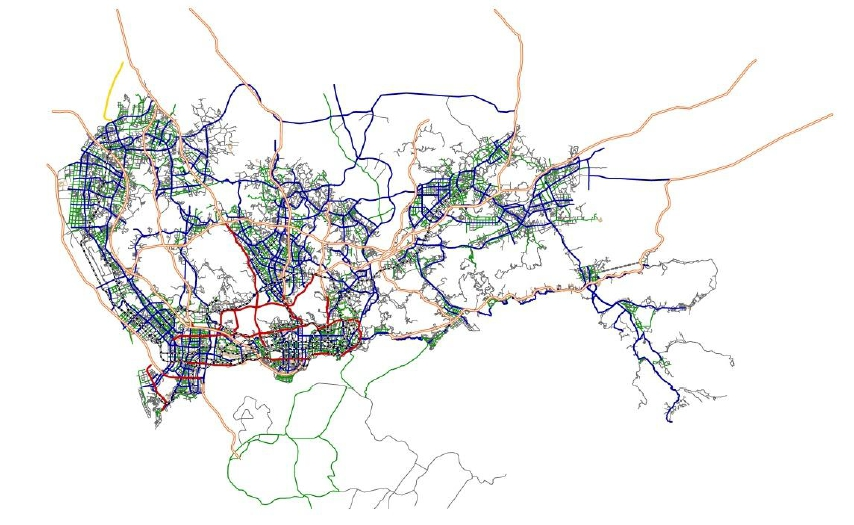
\includegraphics[width=0.85\textwidth]{chp05_盐田大鹏宏观交通模型.jpg}
  \caption{盐田、大鹏宏观交通模型\label{fig:chp05_盐田大鹏宏观交通模型} }
\end{figure}

\item 利用 PTV VISUM 多选功能,选择范围内的路段,如图\ref{fig:chp05_宏观模型中的盐田大鹏中观范围路段}所示。
\begin{figure}[!ht]
  \centering
  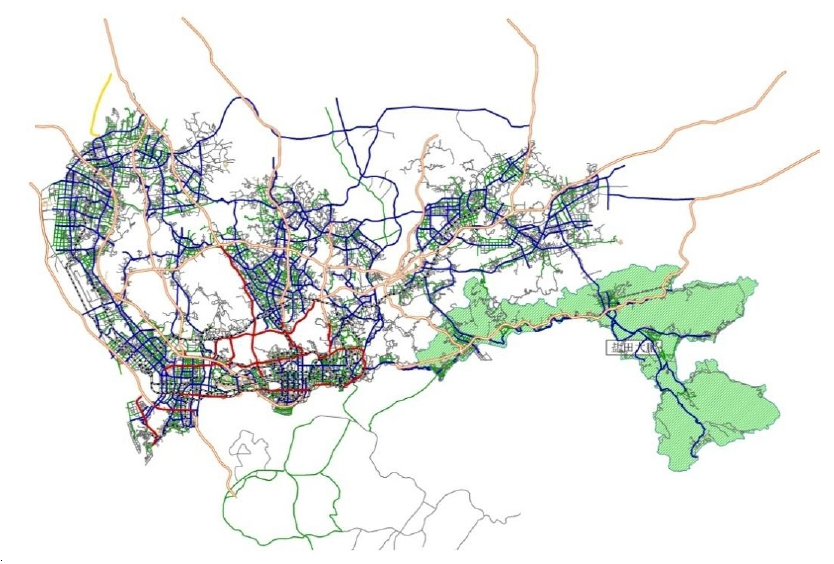
\includegraphics[width=0.85\textwidth]{chp05_宏观模型中的盐田大鹏中观范围路段.jpg}
  \caption{宏观模型中的盐田、大鹏中观范围路段\label{fig:chp05_宏观模型中的盐田大鹏中观范围路段} }
\end{figure}

\item 利用 PTV VISUM 的 Subnetwork Generator 功能,截取盐田、大鹏路
网,结果如图\ref{fig:chp05_从宏观模型截取的盐田大鹏现状路网}所示。
\begin{figure}[!ht]
  \centering
  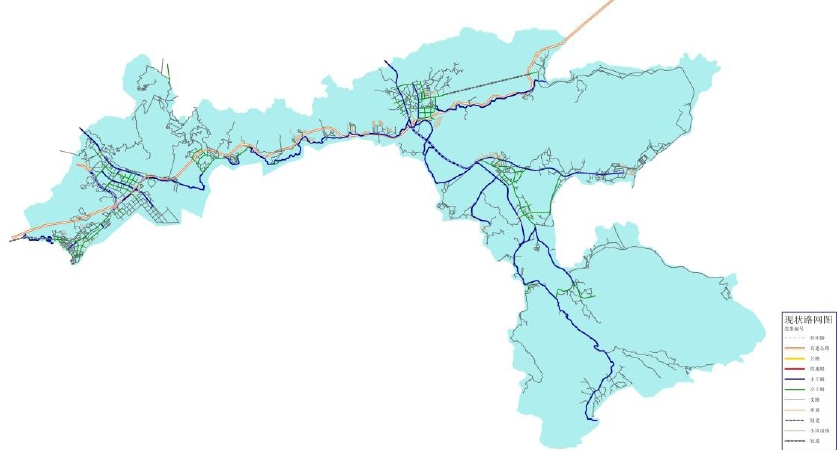
\includegraphics[width=0.85\textwidth]{chp05_从宏观模型截取的盐田大鹏中观现状模型路网.jpg}
  \caption{从宏观模型截取的盐田大鹏现状路网\label{fig:chp05_从宏观模型截取的盐田大鹏现状路网} }
\end{figure}

\item 删减外围路段,得到盐田、大鹏的中观交通基础模型包含路段约861条,如图所示。
\begin{figure}[!ht]
  \centering
  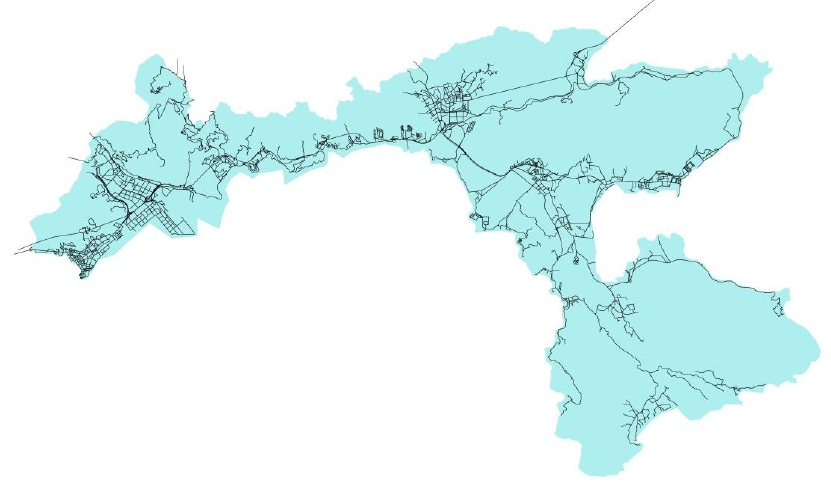
\includegraphics[width=0.85\textwidth]{chp05_盐田大鹏中观现状模型道路网.jpg}
  \caption{盐田、大鹏中观现状模型道路网\label{fig:chp05_盐田大鹏中观现状模型道路网} }
\end{figure}
\end{nbeae}

\subsection{交叉口渠化数据输入}
根据设计报告,在盐田、大鹏中观现状模型道路网的基础上,根据地形图、交叉口渠化信息录入交叉口渠化数据。

\subsubsection{立交信息细化}
根据地形图及相关 CAD 数据中的立交线性,绘制立交拓扑结构,并对结构中的每一个节点的转向关系进行设置。
以盐田区的深盐路-梧桐山大道立交为例,其实际立交形式如图\ref{fig:chp05_深盐路-梧桐大道立交节点}所示。

\begin{figure}[!ht]
  \centering
  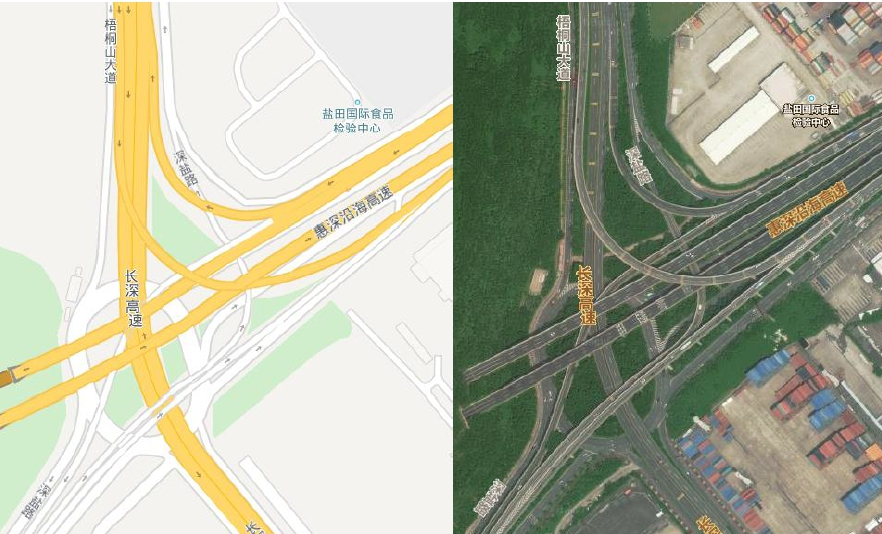
\includegraphics[width=\textwidth]{chp05_深盐路-梧桐大道立交节点.jpg}
  \caption{深盐路-梧桐大道立交节点\label{fig:chp05_深盐路-梧桐大道立交节点} }
\end{figure}

据此,在 VISUM 软件中,绘制深盐路-梧桐大道立交的拓扑结构如图\ref{fig:chp05_深盐路-梧桐大道立交拓扑结构}所示。

\begin{figure}[!ht]
  \centering
  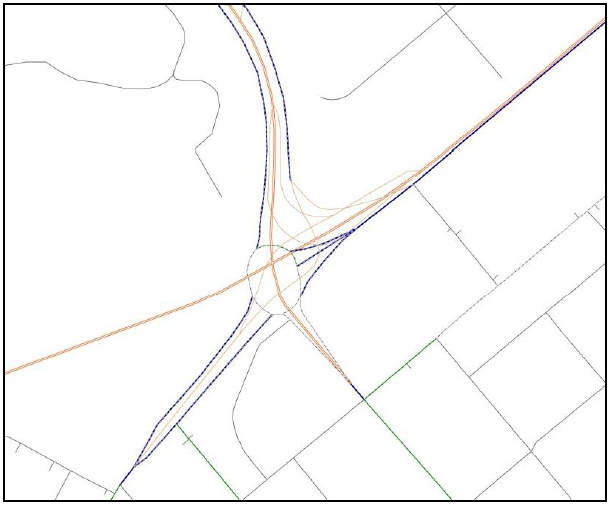
\includegraphics[width=0.6\textwidth]{chp05_深盐路-梧桐大道立交拓扑结构.jpg}
  \caption{深盐路--梧桐大道立交拓扑结构\label{fig:chp05_深盐路-梧桐大道立交拓扑结构} }
\end{figure}

完成拓扑绘制以后,要定义立交中各节点的转向关系,将不允许或不能够通
行车辆的转向禁止。需要对立交中的所有节点一一定义其转向关系,如图\ref{fig:chp05_节点转向关系编辑}所示。
盐田、大鹏现状中观模型共包含各类立交13 个。

\begin{figure}[!ht]
  \centering
  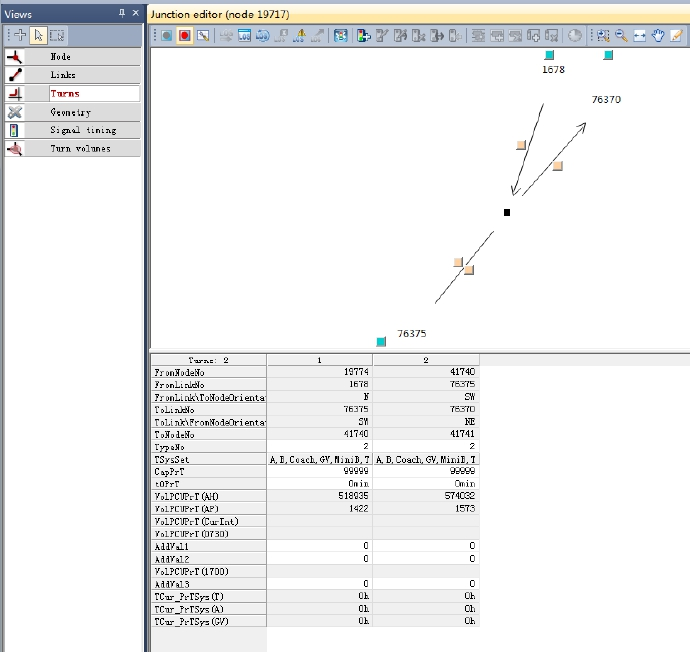
\includegraphics[width=0.6\textwidth]{chp05_节点转向关系编辑.jpg}
  \caption{节点转向关系编辑\label{fig:chp05_节点转向关系编辑} }
\end{figure}

\subsubsection{节点渠化输入}
将交叉口渠化信息,包括交叉口车道数、是否有展宽、各车道的转向信息等
录入到中观现状模型中。 本次先以实际勘探的方式判断其他交叉口渠化信息,若
实勘不清楚,再通过百度街景观察,然后把每个交叉口具体的渠化信息,做成
excel 表格录入到 EXCEL 表(见图\ref{fig:chp05_渠化录入信息表}),最后通过二次程序开发,统一生成 PTV 的渠化模
板,统一录入到 PTV 模型中, 示例如图\ref{fig:chp05_深盐路和沙深路交叉口渠化数据录入示例}所示。

\begin{figure}[!ht]
  \centering
  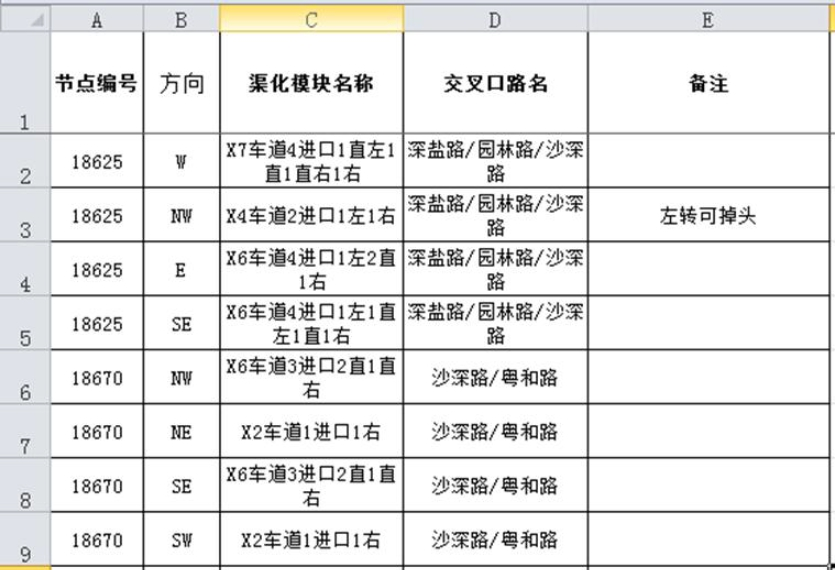
\includegraphics[width=0.7\textwidth]{chp05_渠化录入信息表.jpg}
  \caption{渠化录入信息表\label{fig:chp05_渠化录入信息表} }
\end{figure}

\begin{figure}[!ht]
  \centering
  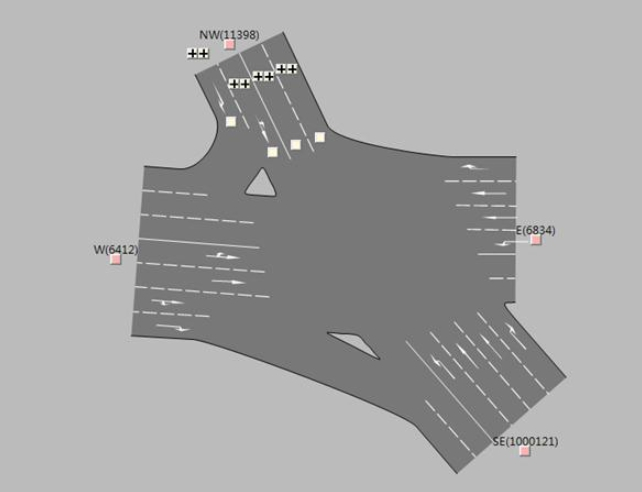
\includegraphics[width=0.6\textwidth]{chp05_深盐路和沙深路交叉口渠化数据录入示例.jpg}
  \caption{深盐路和沙深路交叉口渠化数据录入示例\label{fig:chp05_深盐路和沙深路交叉口渠化数据录入示例} }
\end{figure}

\subsection{交叉口信控数据输入}
根据信号控制机平日时段表(见图\ref{fig:chp05_信号控制机平日时段表}),索引高峰小时(早高峰 7:45-8:45,晚高峰
17:30-18:30)的信号控制相位状态、相位数、配时方案编号以及周期长度。

\begin{figure}[!ht]
  \centering
  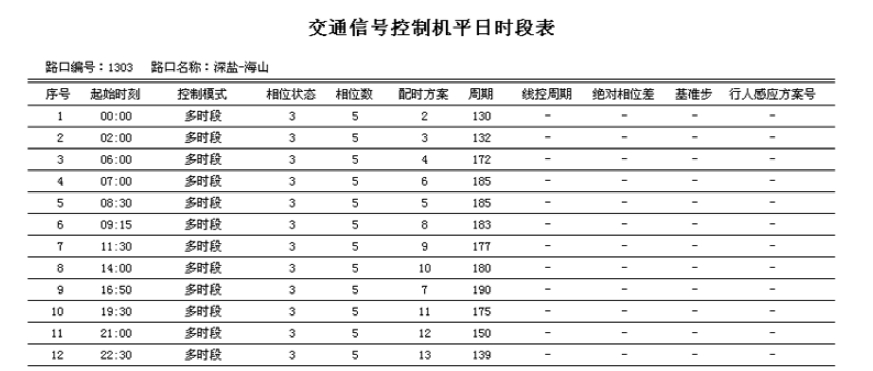
\includegraphics[width=\textwidth]{chp05_信号控制机平日时段表.jpg}
  \caption{信号控制机平日时段表\label{fig:chp05_信号控制机平日时段表} }
\end{figure}

根据前表索引到的信号控制相位状态、相位数、配时方案编号以及周期长度,
在交通信号控制机方案配时表中查找其实际交通配时方案,并在交通信号控制机
灯色配置表中查找其灯色变化方案(见图\ref{fig:chp05_交通信号控制机方案配时表})。

\begin{figure}[!ht]
  \centering
  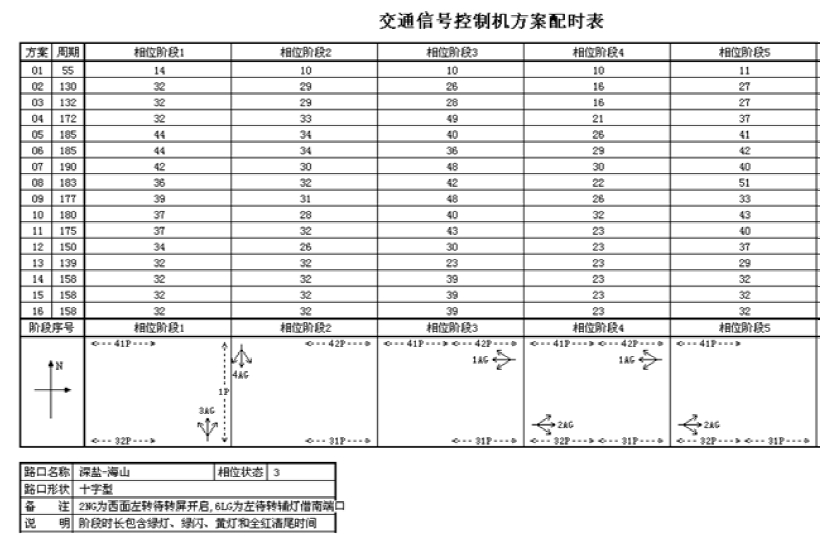
\includegraphics[width=\textwidth]{chp05_交通信号控制机方案配时表.jpg}
  \caption{交通信号控制机方案配时表\label{fig:chp05_交通信号控制机方案配时表} }
\end{figure}

根据前表索引到的配时及灯色方案,在盐田、大鹏中观现状模型中,在相
应的交叉口输入信号配时方案,如图\ref{fig:chp05_信号配时方案输入图}所示。

\begin{figure}[!ht]
  \centering
  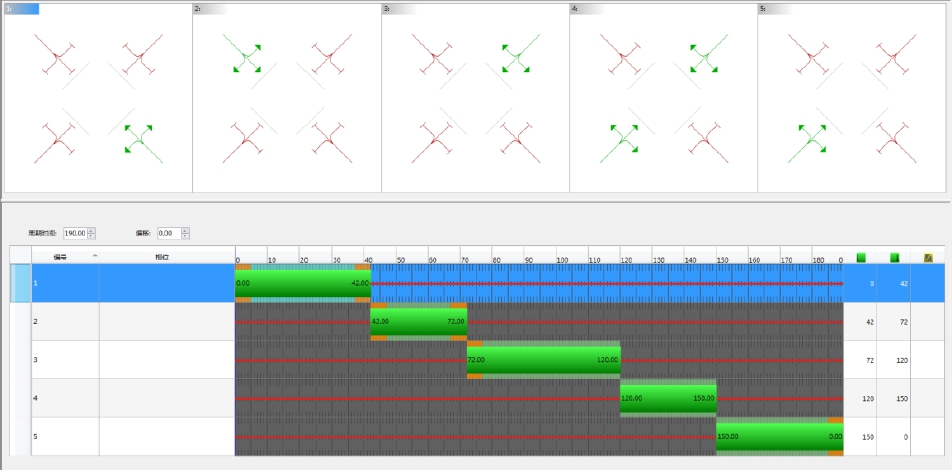
\includegraphics[width=\textwidth]{chp05_信号配时方案输入图.jpg}
  \caption{信号配时方案输入图\label{fig:chp05_信号配时方案输入图} }
\end{figure}

盐田、大鹏中观现状模型的信号控制交叉口分布如图\ref{fig:chp05_盐田大鹏中观现状模型信号控制交叉口分布图}所示,共计 81 个。

\begin{figure}[!ht]
  \centering
  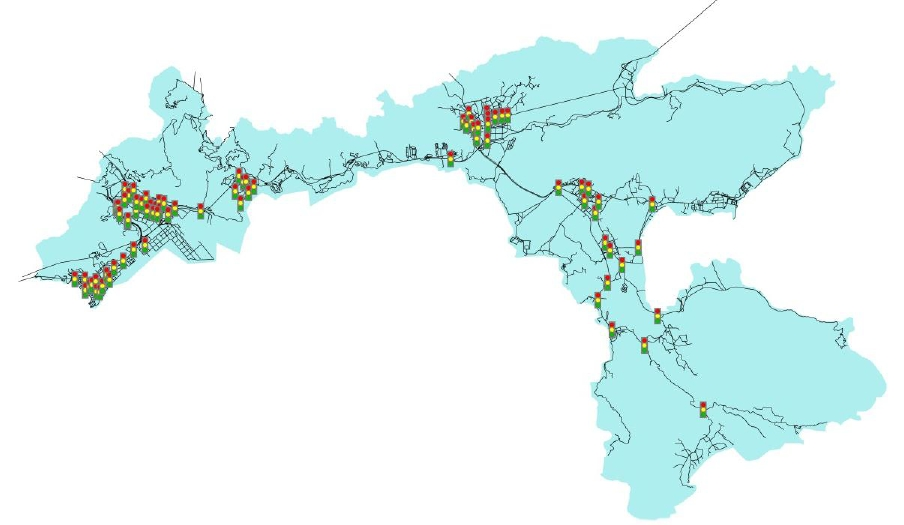
\includegraphics[width=0.9\textwidth]{chp05_盐田、大鹏中观现状模型信号控制交叉口分布图.jpg}
  \caption{盐田、大鹏中观现状模型信号控制交叉口分布图\label{fig:chp05_盐田大鹏中观现状模型信号控制交叉口分布图} }
\end{figure}

\

\subsection{交通小区拆分}
根据设计报告的交通小区拆分原则,对盐田、大鹏中观现状模型范围所涉及
的所有宏观交通小区进行拆分,共计拆分得到 421 个中观
内部交通小区,如图\ref{fig:chp05_盐田大鹏中观内部交通小区图}所示。

\begin{figure}[!ht]
  \centering
  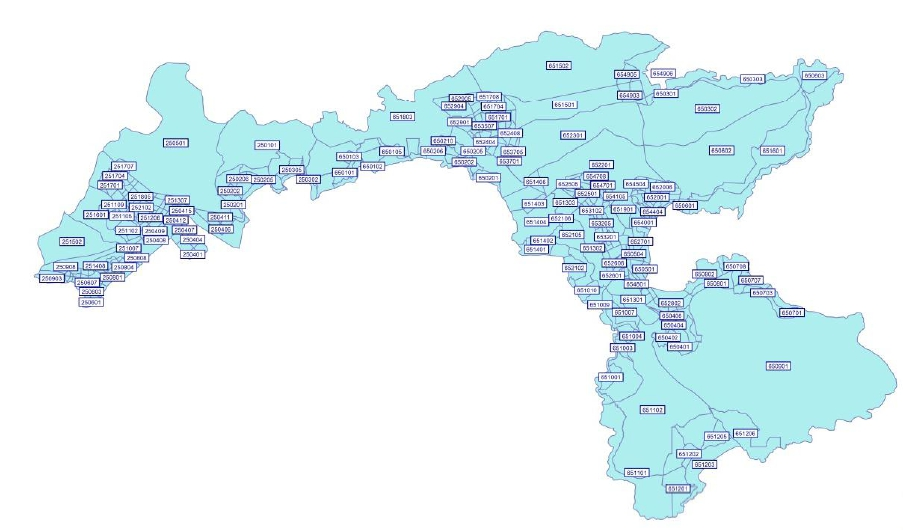
\includegraphics[width=0.9\textwidth]{chp05_盐田大鹏中观内部交通小区图.jpg}
  \caption{盐田、大鹏中观内部交通小区图\label{fig:chp05_盐田大鹏中观内部交通小区图} }
\end{figure}

\subsection{小区连接线绘制}
根据地形图中,各交通小区实际出入口位置分布,绘制交通小区连接线,共绘制了机动车出入口 2034 条连接线,平均每个中观内部
交通小区约 3.9 条小区连接线,如图\ref{fig:chp05_盐田大鹏中观交通小区连接线绘制示例图}}所示。

\begin{figure}[!ht]
  \centering
  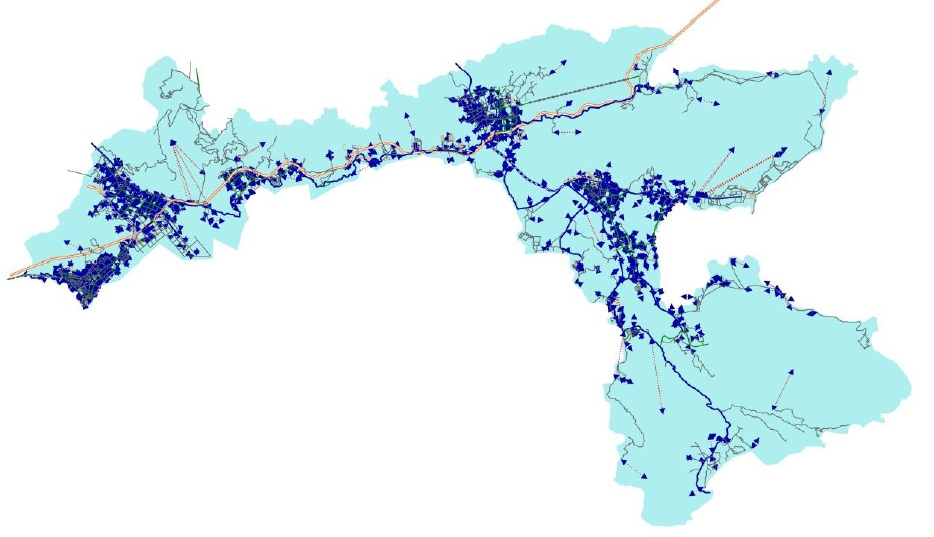
\includegraphics[width=0.9\textwidth]{chp05_盐田大鹏中观交通小区连接线绘制示例图.jpg}
  \caption{盐田、大鹏中观交通小区连接线绘制示例图 \label{fig:chp05_盐田大鹏中观交通小区连接线绘制示例图} }
\end{figure}

\subsection{外部交通小区设置}
根据盐田、大鹏外围通道与周边区域的衔接情况,按每个主、次干道单独一
个外部交通小区的原则,设置盐田、大鹏中观现状模型外部交通小区。 盐田、大
鹏中观现状模型共包含 11 个外部交通小区,编号范围为 1000000-1000010,如
图\ref{fig:chp05_盐田大鹏中观现状模型外部交通小区分布图}所示。

\begin{figure}[!ht]
  \centering
  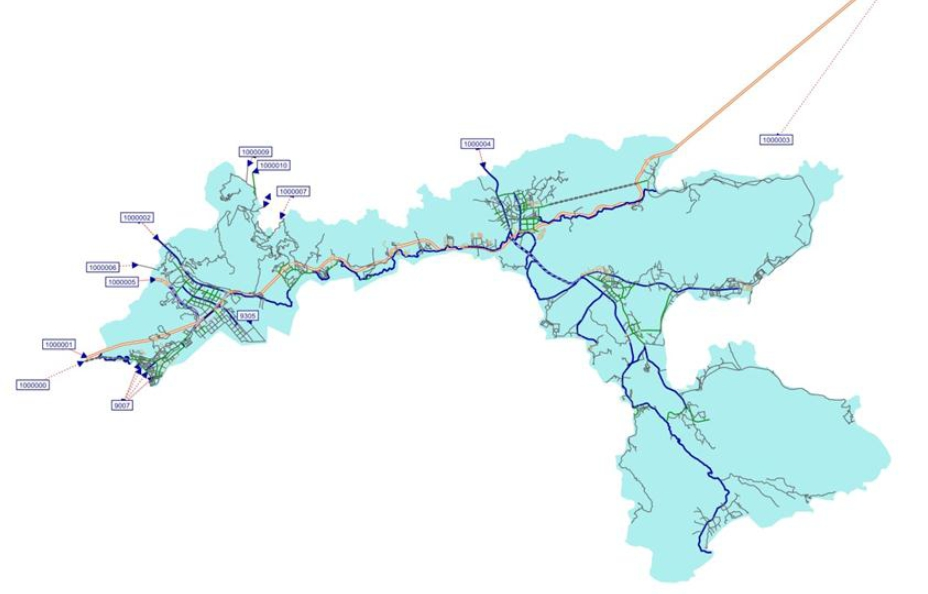
\includegraphics[width=0.9\textwidth]{chp05_盐田大鹏中观现状模型外部交通小区分布图.jpg}
  \caption{盐田、大鹏中观现状模型外部交通小区分布图\label{fig:chp05_盐田大鹏中观现状模型外部交通小区分布图} }
\end{figure}

\subsection{路网检查}
完成上述路网定义后,需要对路网进行检查,如图所示:

\begin{figure}[!ht]
  \centering
  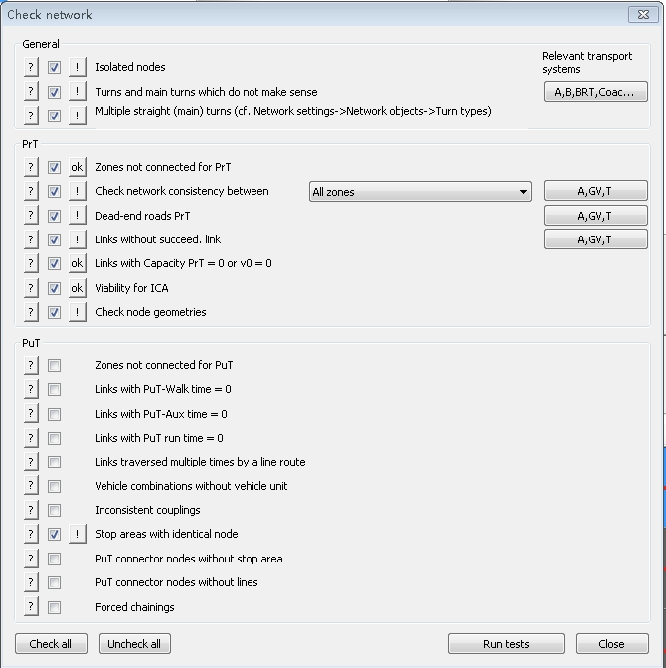
\includegraphics[width=0.65\textwidth]{chp05_中观模型路网检查.jpg}
  \caption{中观模型路网检查\label{fig:chp05_中观模型路网检查} }
\end{figure}

路网检查经常遇到的错误及处理方法如下:

\smalltitle{孤立点清理}

孤立点是指对模型路网无用的节点,该节点未连接任何路段、小区连接线、
公交站点。

对于盐田、大鹏中观交通模型路网中的孤立点,全部删除。

\smalltitle{转向与车道匹配处理}

由于设置的渠化时,某些禁止通行向的转向未关闭,因此需要对其转向进行
处理。

对于盐田、大鹏中观交通模型路网中的不匹配问题,在查核时先确认节点的
渠化是否正确,若正确则关闭转向(即设置转向的交通系统集为空),若不正确
则修正渠化,再重复查核。

\smalltitle{多直行处理}

对于一个交叉口的某一进口车道存在多个直行方向(直行、右转、左转的默
认设置是由 VISUM 根据方向自动生成的)的情况,需要进行处理,每个进口方向仅允许一个直行方向(可设置多个左转或右转方向)。这中情况多存在于畸形
交叉口或高架道路的匝道与地面的衔接处。

对于盐田、大鹏中观交通模型路网中的多直行问题,需判断多个直行中哪一
个才是真正的直行,将其他若干个“非直行的直行车道”改为相应的左转或右转方向。

\smalltitle{小区与路网的连接关系校核}

校核交通小区与路网是否衔接。

在盐田、大鹏中观交通模型路网中,由于交通小区和路网的连接关系继承现
状模型的设置,因此不存在此问题。

\smalltitle{尽端道路处理}

尽端道路是指某一条道路的一段未连接其他道路,同时未连接小区连接线。

对于盐田、大鹏中观交通模型路网中存在的尽端道路问题,一一对其进行查
核,判断其可能存在的问题和处理方法如下:

\begin{itemize}
\item[\XSolidBrush] 是否存在两条道路应该相交,而实际没有连接到同一点的情况?
\item[\Checkmark] 将同一位置的若干个节点进行合并,使路网之间拓扑能够相连接。
\item[\XSolidBrush] 是否存在应该连小区连接线而未连接的情况?
\item[\Checkmark] 将周边小区的小区连接线连接至该路段的尽端。
\item[\XSolidBrush] 是否存在对模型无用的路段(或与其他路段均无连接关系的局部路网)?
\item[\Checkmark] 删除这些无用的路段或与其他路段均无连接关系的局部路网。
\end{itemize}

\smalltitle{未成功连接道路处理}

未成功连接的道路是指道路从拓扑结构上是连接了其他道路,但由于交通系
统集或通行能力、车道数等的设置,实际上车辆无法通过该路段的一端进入其他
道路或小区连接线。

对于盐田、大鹏中观交通模型路网中存在的未成功连接道路,一一对其进行
查核,判断其可能存在的问题和处理方法如下:

\begin{itemize}
\item[\XSolidBrush] 是否存在进口道路允许某种方式通行,而出口道路不允许这种方式
通行的情况?
\item[\Checkmark] 梳理是否应该允许该方式通行,设置相同的交通系统集。
\item[\XSolidBrush] 是否存在道路允许某种方式通行,而交叉口转向或渠化不允许这种
方式通行的情况?
\item[\Checkmark] 查核并修正交叉口转向或渠化设置。
\end{itemize}

\smalltitle{通行能力为零的路段处理}

通行能力为零的路段是指路段允许通行某种交通方式,但通行能力却设为零,
两者出现矛盾。

对于盐田、大鹏中观交通模型路网中存在的通行能力为零的路段,查核其是
否允许车辆通行,若允许则根据道路等级修改通行能力,若不允许则关闭该交通
系统集。

\smalltitle{ICA 计算设置校核}

校核信号控制交叉口,节点渠化和信号控制设定是否准确。该判断为逻辑判
断,即信号控制设置存在逻辑错误时提示。

对于盐田、大鹏中观交通模型路网中存在的 ICA 计算设置错误,一一将其
修正。(由于 ICA 设置可能存在的问题比较多,在此不一一列举)

\smalltitle{节点渠化校核}

校核非信号控制交叉口渠化是否准确。

对于盐田、大鹏中观交通模型路网中存在的节点渠化问题,一一对其进行查
核,判断其可能存在的问题和处理方法如下:

\begin{itemize}
\item[\XSolidBrush] 是否存在路段允许某种交通方式通行,而车道不允许该交通方式通行的情况?
\item[\Checkmark] 梳理是否应该允许该方式通行,设置相同的交通系统集。
\item[\XSolidBrush] 是否存在车道允许某种交通方式通行,而转向不允许该交通方式通行的情况?
\item[\Checkmark] 梳理是否应该允许该方式通行,设置相同的交通系统集。
\end{itemize}

\smalltitle{完成路网小结}

完成上述校核以后,得到的结果如图\ref{fig:chp05_盐田大鹏中观现状路网校核结果}所示。

\begin{figure}[!ht]
  \centering
  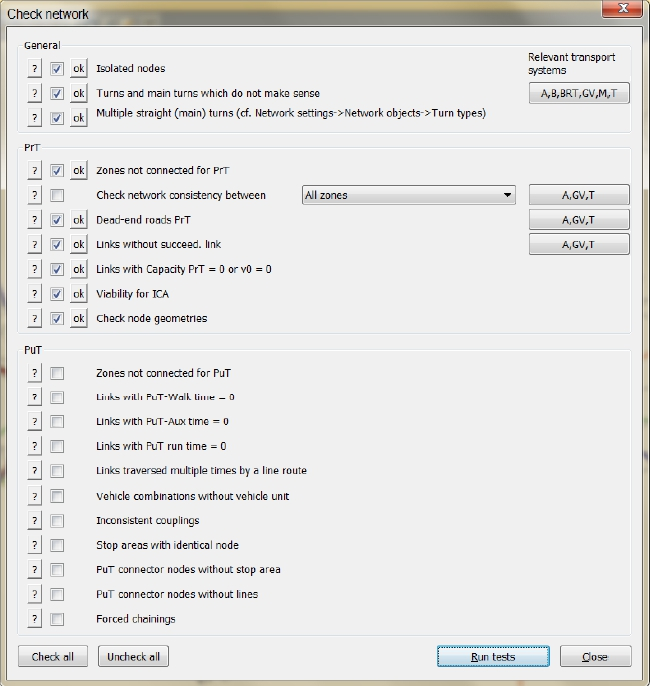
\includegraphics[width=0.7\textwidth]{chp05_盐田大鹏中观现状路网校核结果.jpg}
  \caption{盐田、大鹏中观现状路网校核结果\label{fig:chp05_盐田大鹏中观现状路网校核结果} }
\end{figure}

\section{盐田、大鹏中观现状模型需求计算}
根据宏观现状晚高峰模型计算得到的交通分配结果,利用 VISUM 软件的路
径分析功能,截取盐田、大鹏中观现状模型的晚高峰局部交通 OD。而后在此基
础上进行外部交通小区 OD 整理,以及内部交通小区 OD 拆分。将处理完成以后
的交通 OD 导入到中观现状模型对应的晚高峰模型中,进行交通分配。

\subsection{子路网 OD 截取}
利用 VISUM 软件的 Subnetwork Generator 功能,截取完成交通分配并保存
车流路径的宏观现状交通模型的局部 OD。其操作流程如下:

\begin{nbeae}
\item 打开宏观现状交通模型;
\item 选择菜单 Calculate $\rightarrow$ Subnetwork Generator(局部路网生成器),
弹出以下对话框:

\begin{figure}[!ht]
  \centering
  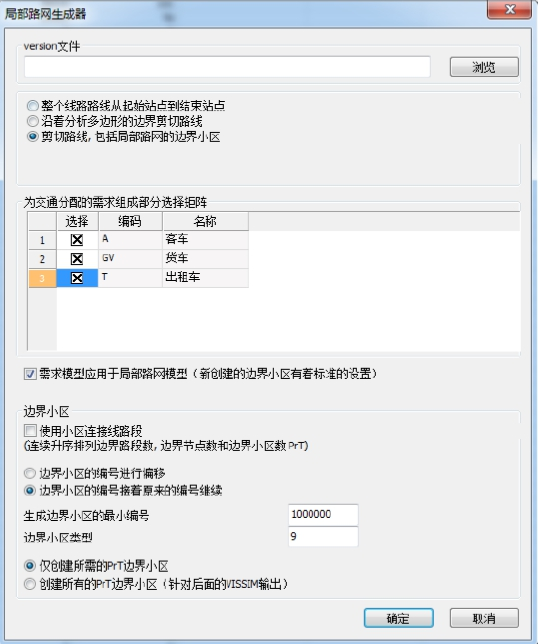
\includegraphics[width=0.5\textwidth]{chp05_SubnetworkGenerator对话框.jpg}
  \caption{Subnetwork Generator对话框\label{fig:chp05_Subnetwork Generator对话框} }
\end{figure}

\item 选择所要截取的 OD 矩阵,并选择确定;
\item 打开截取所获得的子路网模型,并得到各方式OD矩阵(83$\times$83)。
\end{nbeae}

在盐田、大鹏中观现状模型建模过程中,从宏观现状模型里截取了小汽车
( A)、出租车( T)以及货车( GV)三种方式的局部 OD,并在 Excel 表中,对
小汽车和出租车方式的 OD 进行了合并(相加),得到汽车方式出行 OD(见图\ref{fig:chp05_从宏观模型截取得到的中观局部OD矩阵})。

\begin{figure}[!ht]
  \centering
  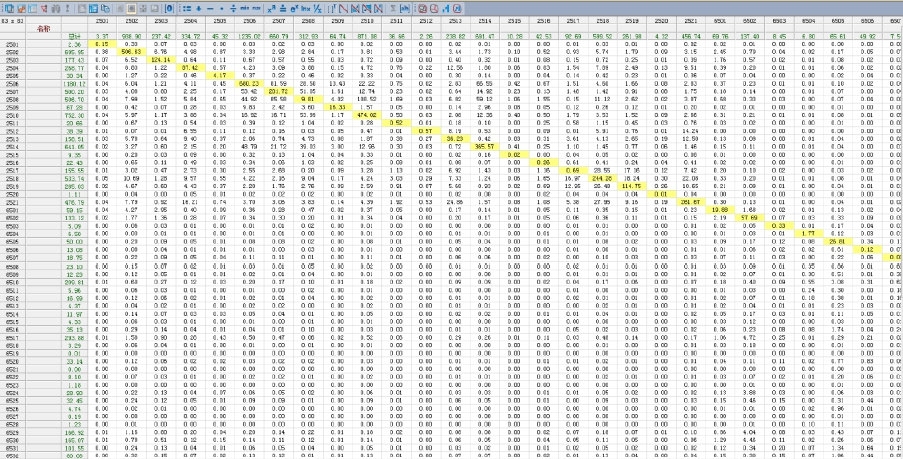
\includegraphics[width=0.8\textwidth]{chp05_从宏观模型截取得到的中观局部OD矩阵.jpg}
  \caption{从宏观模型截取得到的中观局部OD矩阵\label{fig:chp05_从宏观模型截取得到的中观局部OD矩阵} }
\end{figure}

\subsection{外部 OD 整理}
由于从宏观模型截取得到的外部交通小区(以下简称“宏观外部小区”) 共 11
个, 与中观现状模型的外部交通小区(以下简称“中观外部小区”)一致,因此宏
观外部小区与中观外部小区直接对应。

完成上述工作以后,即得到整理之后的中观小区 83$\times$83 OD 矩阵:

\begin{figure}[!ht]
  \centering
  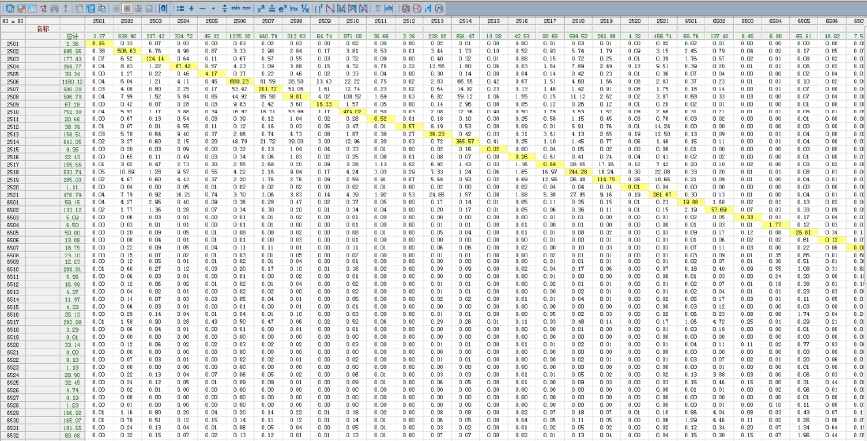
\includegraphics[width=0.8\textwidth]{chp05_宏观截取矩阵初步合并.jpg}
  \caption{宏观截取矩阵初步合并\label{fig:chp05_宏观截取矩阵初步合并} }
\end{figure}

\subsection{OD 拆分计算}
根据建筑普查的数据,统计得到中观现状模型各交通小区各类用地的建筑量数据,按宏观模型的产生吸引率,
计算各中观现状模型交通小区的产生吸引量,并以此计算各交通小区的拆分比率。

\begin{figure}[!ht]
  \centering
  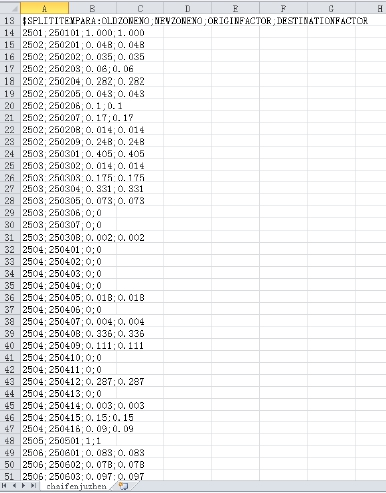
\includegraphics[width=0.4\textwidth]{chp05_中观现状模型各交通小区拆分比率示例.jpg}
  \caption{中观现状模型各交通小区拆分比率示例\label{fig:chp05_中观现状模型各交通小区拆分比率示例} }
\end{figure}

利用 PTV 软件的矩阵拆分功能(见图\ref{fig:chp05_中观现状模型矩阵拆分操作}),将合并后的 83$\times$83 矩阵拆分为 434$\times$434 矩阵,拆分结果如图\ref{fig:chp05_中观现状模型矩阵拆分结果}所示。

\begin{figure}[!ht]
  \centering
  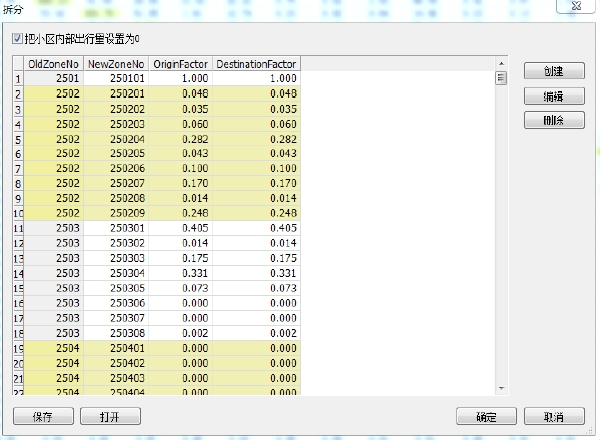
\includegraphics[width=0.6\textwidth]{chp05_中观现状模型矩阵拆分操作.jpg}
  \caption{中观现状模型矩阵拆分操作\label{fig:chp05_中观现状模型矩阵拆分操作} }
\end{figure}

\begin{figure}[!ht]
  \centering
  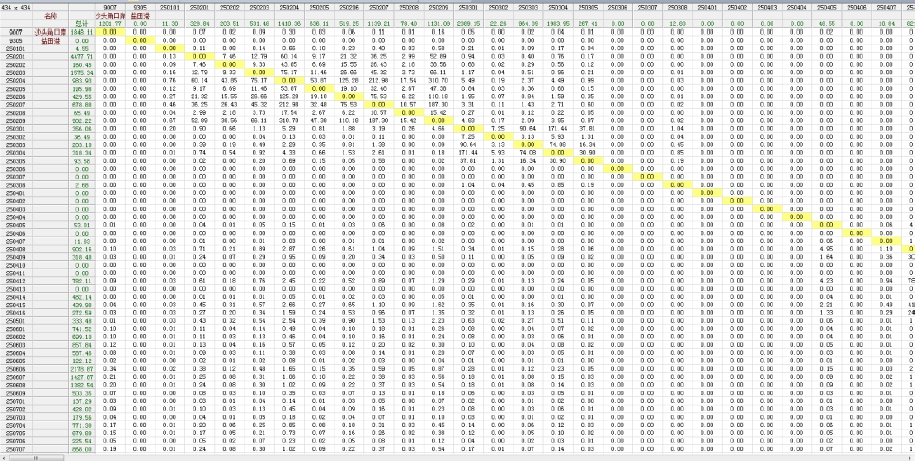
\includegraphics[width=\textwidth]{chp05_中观现状模型矩阵拆分结果.jpg}
  \caption{中观现状模型矩阵拆分结果\label{fig:chp05_中观现状模型矩阵拆分结果} }
\end{figure}

\subsection{交通分配}
\smalltitle{设置节点阻抗计算}

在 VISUM 软件的菜单中,选择 Calculate $\rightarrow$ General procedure settings,打开
分配设置界面。选中 PrT settings / Node Impedances,设置节点阻抗计算方法
(见图\ref{fig:chp05_节点阻抗计算方法设置界面})。

\begin{figure}[!ht]
  \centering
  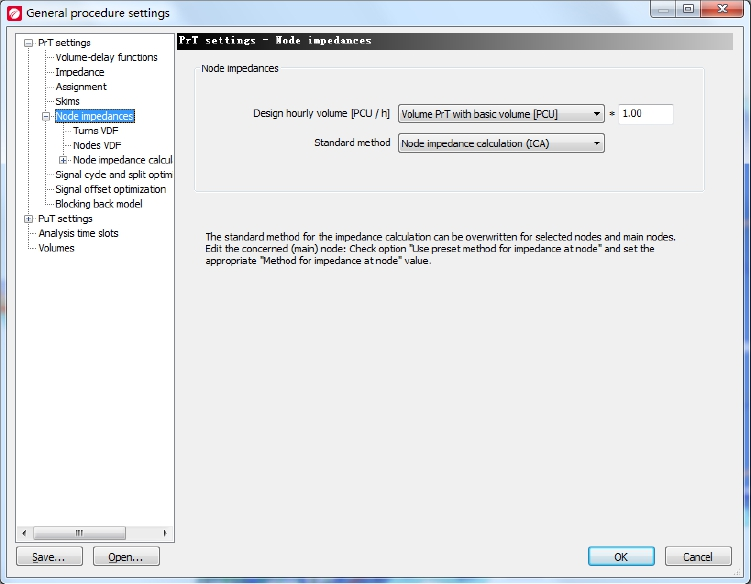
\includegraphics[width=0.7\textwidth]{chp05_节点阻抗计算方法设置界面.jpg}
  \caption{节点阻抗计算方法设置界面\label{fig:chp05_节点阻抗计算方法设置界面} }
\end{figure}


在盐田、大鹏中观现状模型建模中,设置 Design hourly volume [PCU/h]为
Volume PrT with basic volume [PCU]*1.00(分配的已经是 pcu 矩阵了,无需进行
转换),设置 Standard method 为 Node impedance calculation (ICA) (计算节点阻抗)。

然后,在 Node impedances / Node impedance calculation (ICA)下,设置不同
交叉口类型的 ICA 计算方法。 ICA 基本设置为: tCur update 的方式为 Before and
during assignment(且只针对激活的节点进行更新);在 U-turn 的处理上,设置忽
略 U-turn 的影响; Time interval 设置为 15min;同时让软件自动输出 Excel 算表
(见图\ref{fig:chp05_ICA计算总体设置界面})。

\begin{figure}[!ht]
  \centering
  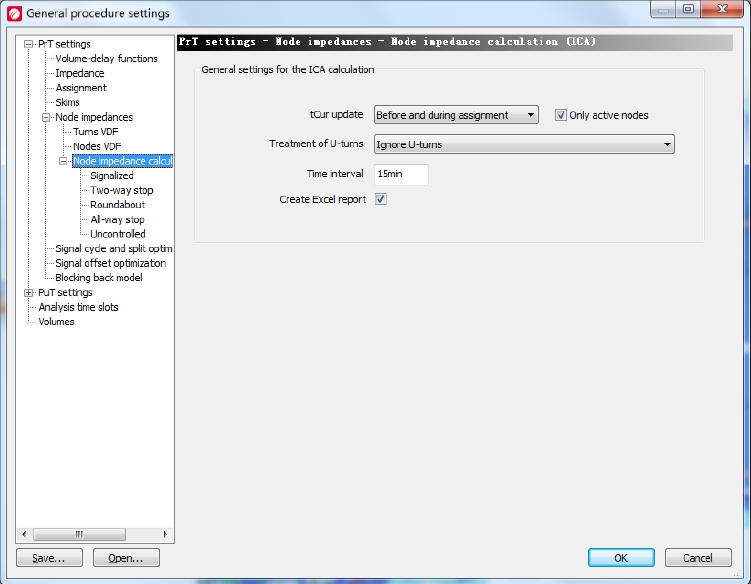
\includegraphics[width=0.7\textwidth]{chp05_ICA计算总体设置界面.jpg}
  \caption{ICA计算总体设置界面\label{fig:chp05_ICA计算总体设置界面} }
\end{figure}

对于信号控制交叉口,其设置如下:计算标准采用 HCM 2000 标准,最大 tCur
设置为 10min, Queue length percentile 设置为 90\%,饱和流率分别设为 1900、1600和 1600
(见图\ref{fig:chp05_信号控制交叉口设置界面})。

\begin{figure}[!ht]
  \centering
  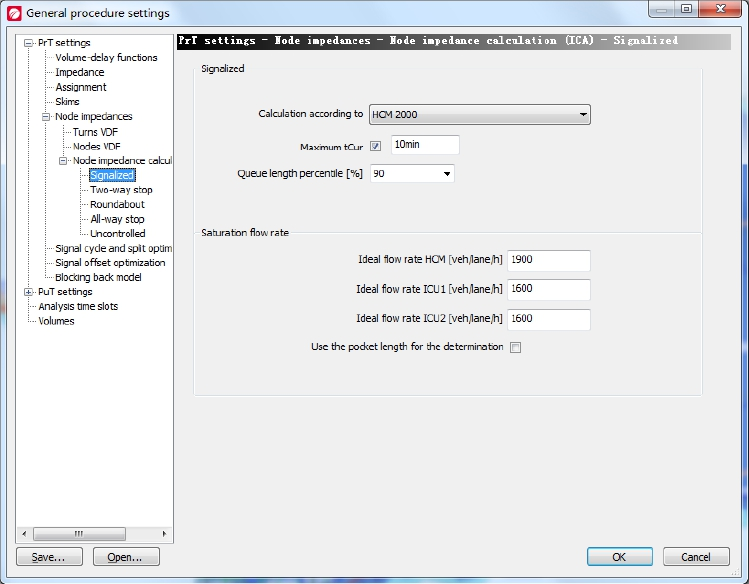
\includegraphics[width=0.7\textwidth]{chp05_信号控制交叉口设置界面.jpg}
  \caption{信号控制交叉口设置界面\label{fig:chp05_信号控制交叉口设置界面} }
\end{figure}

对于让行交叉口( Two-way stop 和 All-way stop 相同),其设置如下:计算
标准采用 HCM 2000 标准,最大 tCur 设置为 10min(见图\ref{fig:chp05_让行交叉口设置界面})。

\begin{figure}[!ht]
  \centering
  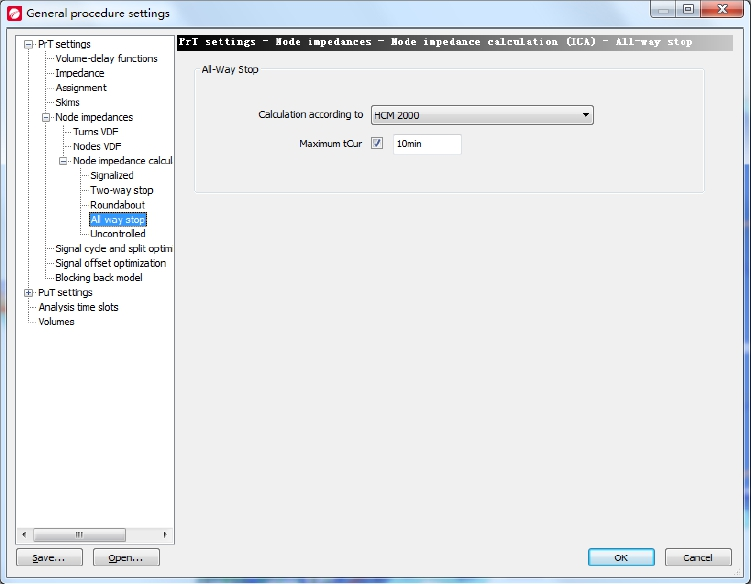
\includegraphics[width=0.7\textwidth]{chp05_让行交叉口设置界面.jpg}
  \caption{让行交叉口设置界面\label{fig:chp05_让行交叉口设置界面} }
\end{figure}

对于非信号控制交叉口,采用 BPR 函数计算延误(见图\ref{fig:chp05_非控制交叉口设置界面})。

\clearpage

\begin{figure}[!ht]
  \centering
  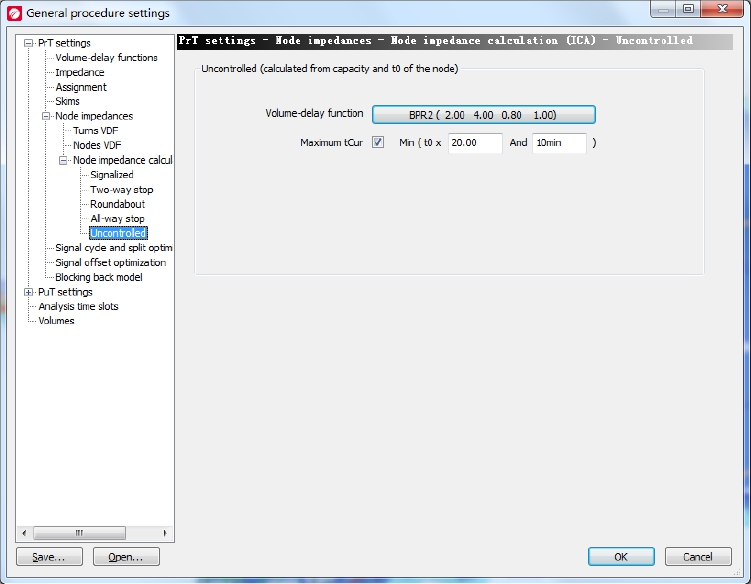
\includegraphics[width=0.7\textwidth]{chp05_非控制交叉口设置界面.jpg}
  \caption{非控制交叉口设置界面\label{fig:chp05_非控制交叉口设置界面} }
\end{figure}
 
\smalltitle{设置背景流量}

在 General procedure settings 中,PrT settings / Assignment 下,设置背景流量。
在截取路网时,已将公交车转换为 PCU 输入到 Link 的 AddValue3 属性中,因此
在模型中设置 AddValue3 作为背景叠加量。

\begin{figure}[!ht]
  \centering
  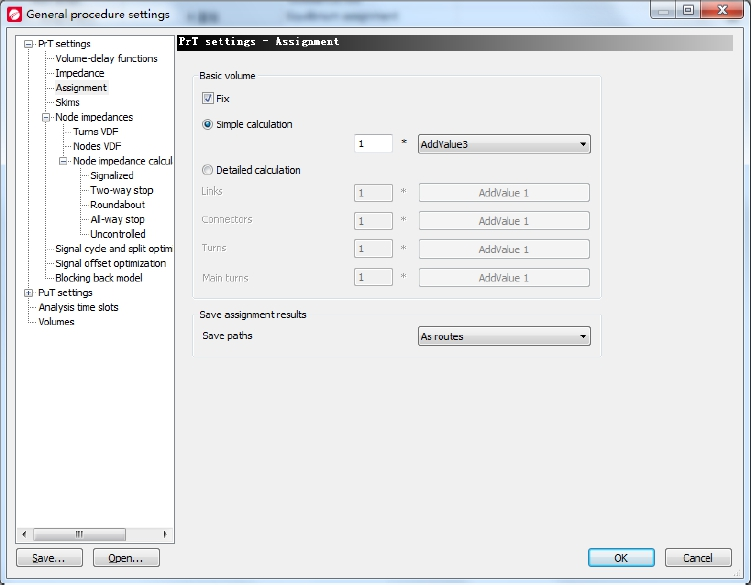
\includegraphics[width=0.7\textwidth]{chp05_背景流量设置界面.jpg}
  \caption{背景流量设置界面\label{fig:chp05_背景流量设置界面} }
\end{figure}

\clearpage

\smalltitle{分配计算步骤}

分配计算步骤包括: 更新节点阻抗和 PrT 方式分配(采用 ICA 均衡分配方法)。

\begin{figure}[!ht]
  \centering
  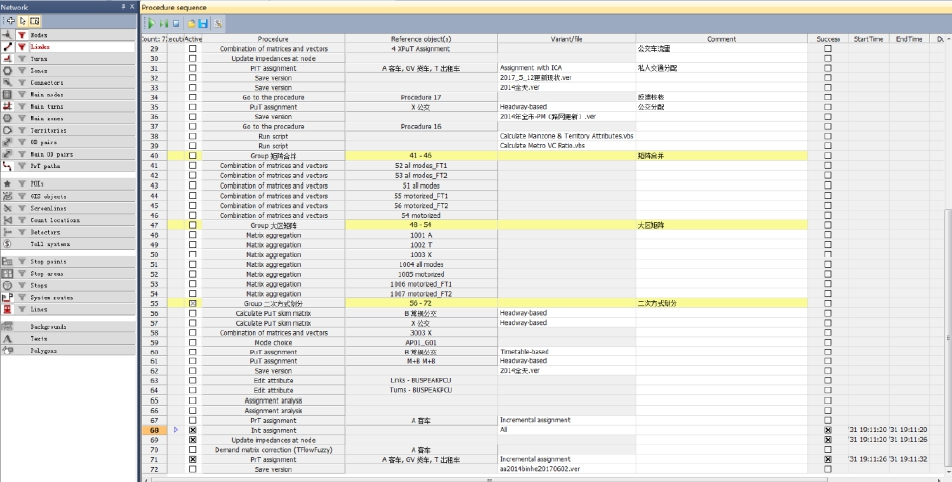
\includegraphics[width=\textwidth]{chp05_分配计算步骤界面1.jpg} \\\vspace{10pt}
  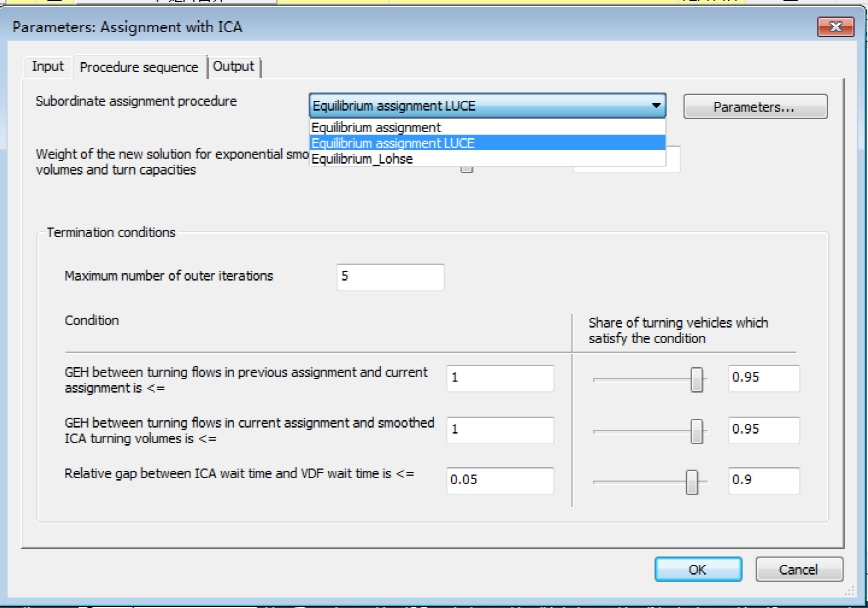
\includegraphics[width=\textwidth]{chp05_分配计算步骤界面2.jpg}
  \caption{分配计算步骤界面\label{fig:chp05_分配计算步骤}}   
\end{figure}

\section{盐田、大鹏中观现状基础模型校验}
根据交通调查得到的流量数据,分别对中观现状晚高峰模型进行校核。

\subsection{交通调查}
模型校核的基准是路段及交叉口的现场调查流量值,为了保证模型精度, 本
次调查方案共涉及 26 个交叉路口, 其中 13 个立交、 8 个 T/Y 型平面交叉口、 5
个十字型平面交叉口(具体点位见图\ref{fig:chp05_调查点位分布图})。调查内容为分车型流量,
另外还包含 3 个路口饱和流量调查,3 个路口排队长度调查,1 个双向路段流量调查。
调查时间:早高峰 7:30-9:30,晚高峰 17:00-19:00,调查日期 2018 年 7 月的周二至周四,调查共计 192 人次。

\begin{figure}[!ht]
  \centering
  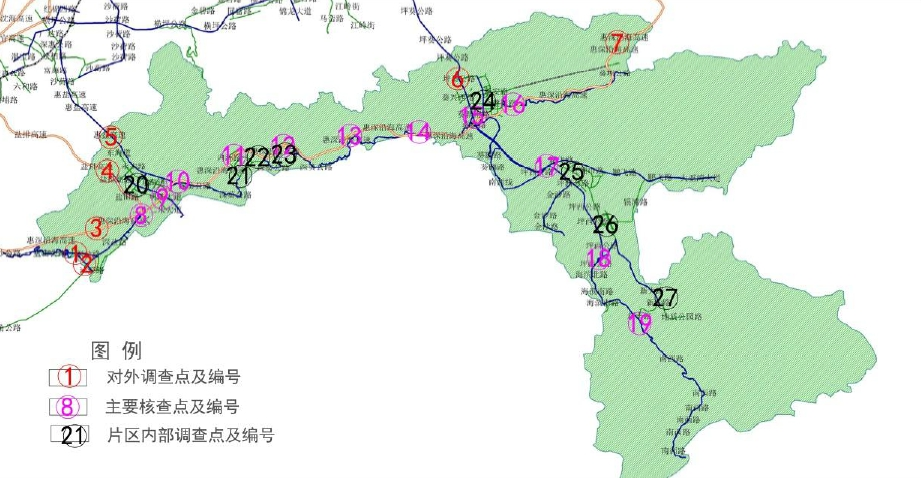
\includegraphics[width=\textwidth]{chp05_调查点位分布图.jpg}
  \caption{调查点位分布图\label{fig:chp05_调查点位分布图} }
\end{figure}

\subsection{校核方法}
本次调查点位足够多,采用 OD 反推的方法进行校核,反推时,限定距离分
布与原矩阵保持一致,外外过境交通不变。具体流程如图\ref{fig:chp05_OD反推设置界面}所示。

\begin{figure}[!ht]
  \centering
  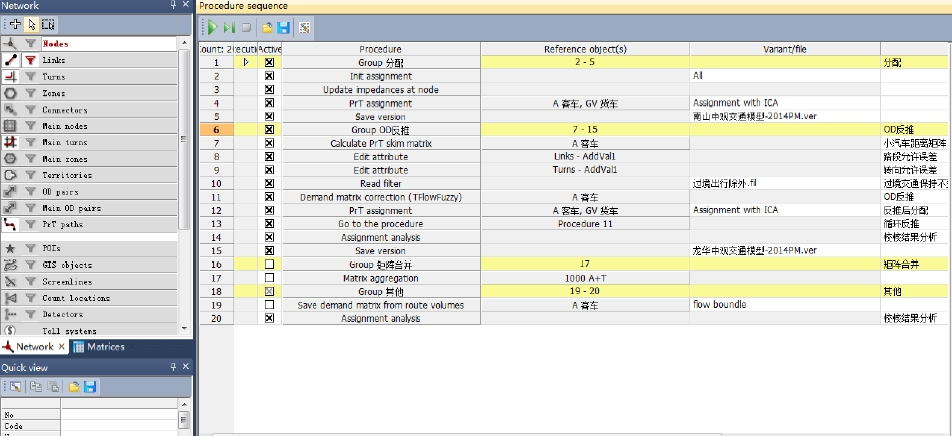
\includegraphics[width=\textwidth]{chp05_OD反推设置界面.jpg}
  \caption{OD反推设置界面\label{fig:chp05_OD反推设置界面} }
\end{figure}

\begin{nbeae}
\item 将调查的路段流量输入到中观现状模型对应 Link 的 Addvalue1 属性
以盐田、大鹏中观现状晚高峰模型为例,其调查路段分布如图\ref{fig:chp05_盐田大鹏中观现状晚高峰模型调查路段分布图}所示。

\begin{figure}[!ht]
  \centering
  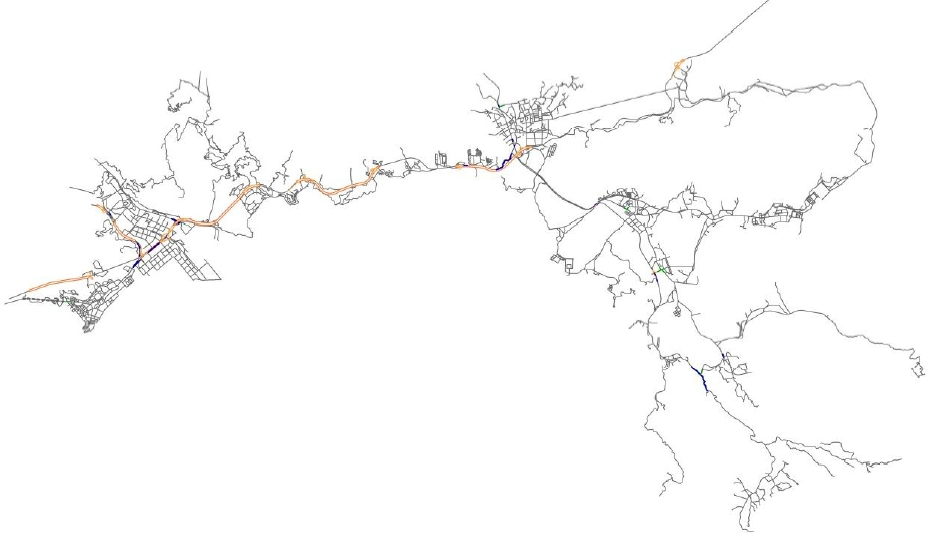
\includegraphics[width=0.9\textwidth]{chp05_盐田大鹏中观现状晚高峰模型调查路段分布图.jpg}
  \caption{盐田、大鹏中观现状晚高峰模型调查路段分布图\label{fig:chp05_盐田大鹏中观现状晚高峰模型调查路段分布图} }
\end{figure}

\clearpage
\item 设置模型分配值允许误差。

\indenttext{开始时,可设置容许位差较大,为调查值的 50\%,模型经过多次迭代后,误
差一般会小于设定值。 Link 的 Addvalue 1 的值为 Sur\_PM\_PV 的 50\%,设置界面如图
\ref{fig:chp05_模型分配容许误差设置界面}所示。}

\begin{figure}[!ht]
  \centering
  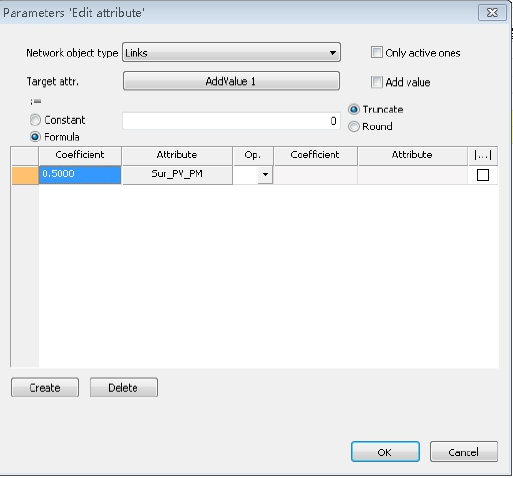
\includegraphics[width=0.9\textwidth]{chp05_模型分配容许误差设置界面.jpg}
  \caption{模型分配容许误差设置界面\label{fig:chp05_模型分配容许误差设置界面} }
\end{figure}

\item 过滤内内出行,内外出行和外内出行部分。

\indenttext{利用 filter 功能(见图\ref{fig:chp05_过滤OD对界面})
过滤出起点在盐田、大鹏或者终点在盐田、大鹏的所有 OD 对,OD 反推时,仅这些 OD 对可以变化,外外 OD 对不可以变。}

\begin{figure}[!ht]
  \centering
  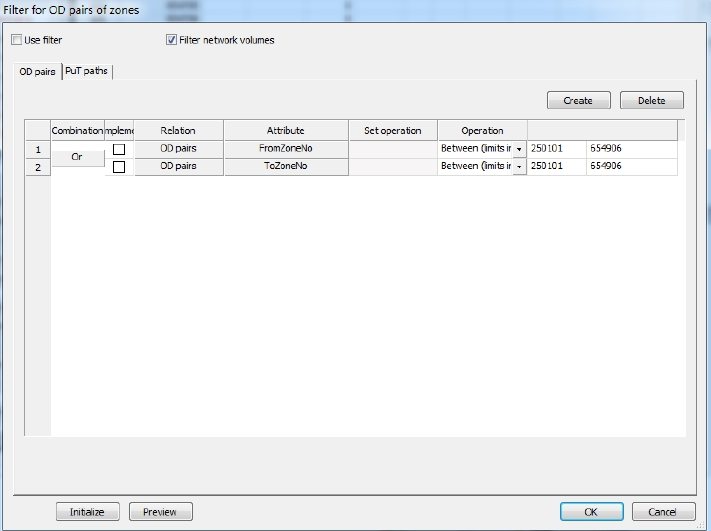
\includegraphics[width=0.7\textwidth]{chp05_过滤OD对.jpg}
  \caption{过滤OD对界面\label{fig:chp05_过滤OD对界面} }
\end{figure}

\item 设置 OD 反推参数。

\indenttext{在 VISUM 软件中,Calculate $\rightarrow$ Procedure sequence 界面中,添加一个 Demand
matrix correction (TFlowFuzzy),如图\ref{fig:chp05_添加TFlowFuzzy界面}所示。 }

\begin{figure}[!ht]
  \centering
  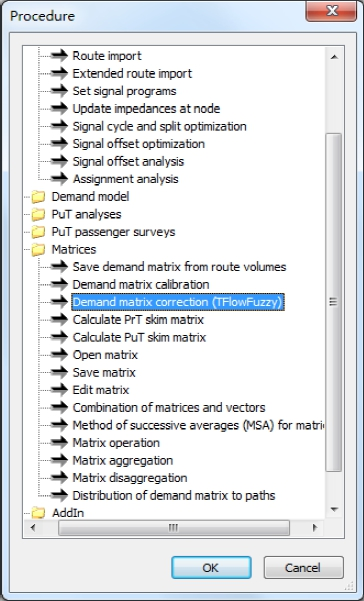
\includegraphics[width=0.4\textwidth]{chp05_添加TFlowFuzzy界面.jpg}
  \caption{添加TFlowFuzzy界面\label{fig:chp05_添加TFlowFuzzy界面} }
\end{figure}

\clearpage

\indenttext{双击 Demand matrix correction (TFlowFuzzy),在基本设置界面勾选“Use only
network object with volume > 0 and counted value > 0”,勾选 Link 下的“Based on counted link volumes” 以 及 “Only active links” , 在流量设置里面选择Sur\_PM\_PV+/- Addvalue 1(见图\ref{fig:chp05_TFlowFuzzy基本设置图})。}

\begin{figure}[!ht]
  \centering
  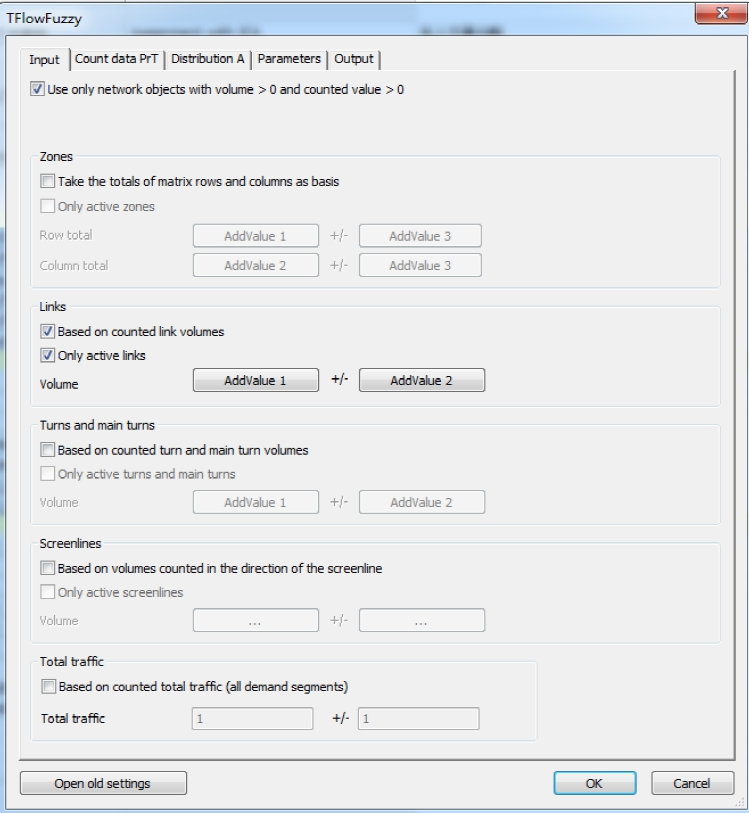
\includegraphics[width=0.7\textwidth]{chp05_TFlowFuzzy基本设置图.jpg}
  \caption{TFlowFuzzy基本设置图\label{fig:chp05_TFlowFuzzy基本设置图} }
\end{figure}

\indenttext{在 Distribution A 标签中,勾选“Based on skim data distribution”,并在 Skim
matrix for classification 中选择距离阻抗矩阵,并在 Classes and shares 下选择
“Preset class limits and derive shares from current matrix”以及“Shares due to the
current demand matrix”(见图\ref{fig:chp05_TFlowFuzzy分布设置图})。}

\begin{figure}[!ht]
  \centering
  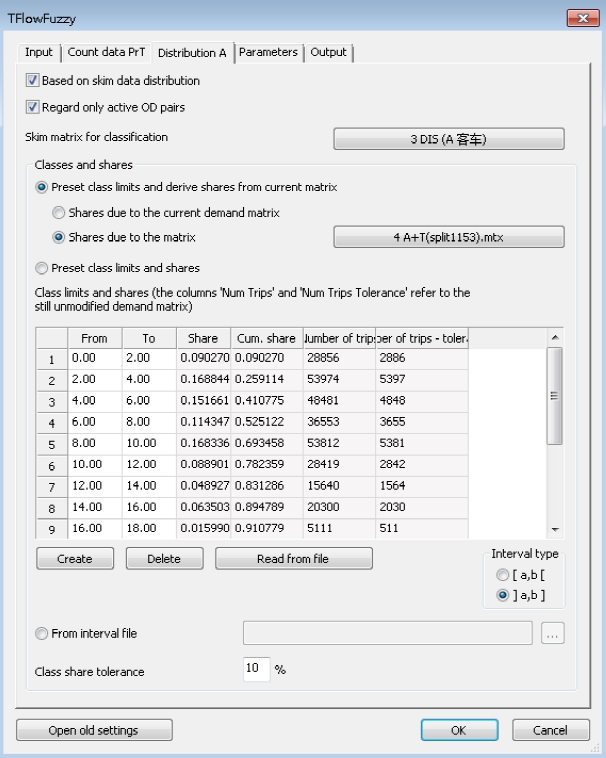
\includegraphics[width=0.65\textwidth]{chp05_TFlowFuzzy分布设置图.jpg}
  \caption{TFlowFuzzy分布设置图\label{fig:chp05_TFlowFuzzy分布设置图} }
\end{figure}
\end{nbeae}

\subsection{校核结果}
以晚高峰模型为例, 根据调查数据,对反推结果进行校核,校核结果如图\ref{fig:chp05_OD反推校核结果图}所示。

\begin{figure}[!ht]
  \centering
  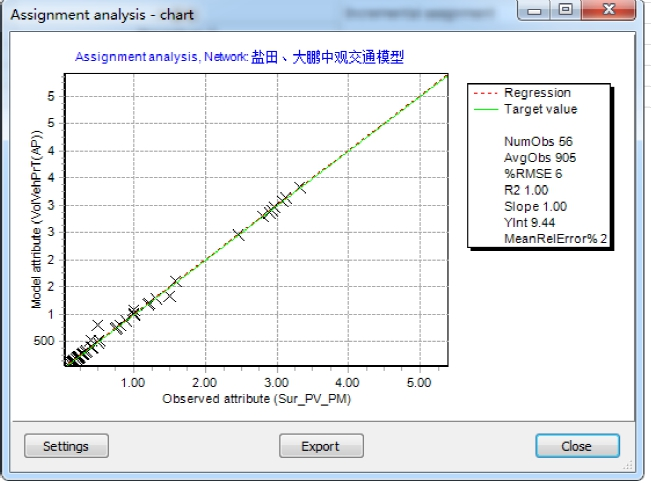
\includegraphics[width=0.7\textwidth]{chp05_OD反推校核结果图.jpg}
  \caption{OD反推校核结果图\label{fig:chp05_OD反推校核结果图} }
\end{figure}

\clearpage

\section{盐田、大鹏中观交通模型成果}
根据设计报告要求,制作各类模型输出图表的配置文件(图为 GPA 文件,
表为 ATT 文件)。下面是各类图表的样例。

\begin{figure}[!ht]
  \centering
  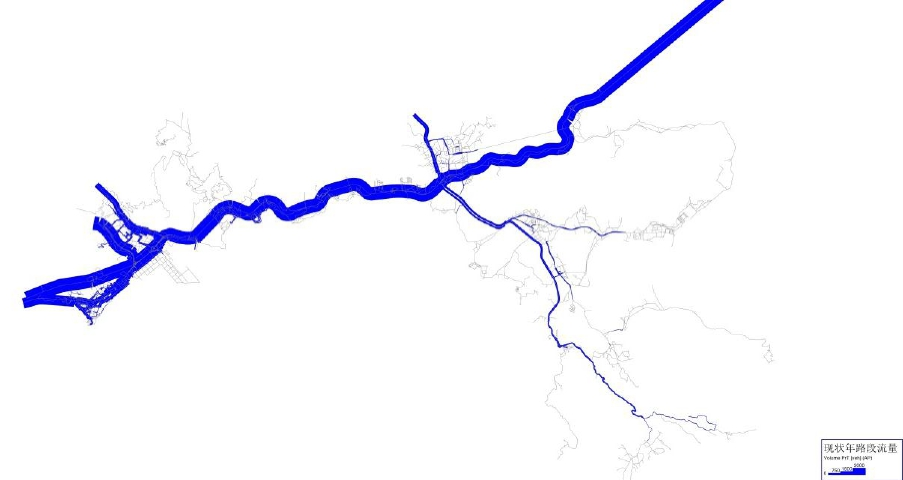
\includegraphics[width=\textwidth]{chp05_现状年盐田大鹏路段流量分布图.jpg}
  \caption{现状年盐田、大鹏路段流量分布图\label{fig:chp05_现状年盐田大鹏路段流量分布图} }
\end{figure}

\begin{figure}[!ht]
  \centering
  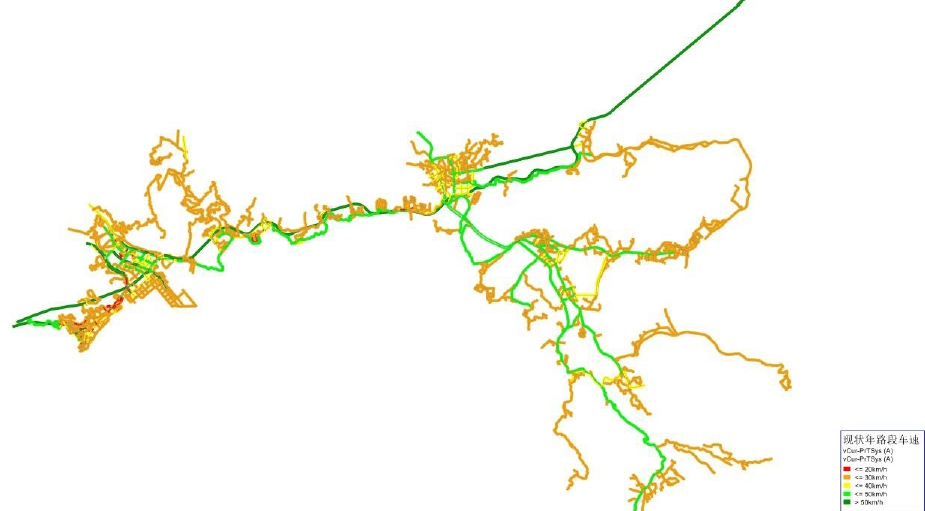
\includegraphics[width=\textwidth]{chp05_现状年盐田大鹏路段速度分布图.jpg}
  \caption{现状年盐田、大鹏路段速度分布图\label{fig:chp05_现状年盐田大鹏路段速度分布图.jpg} }
\end{figure}

\begin{figure}[!ht]
  \centering
  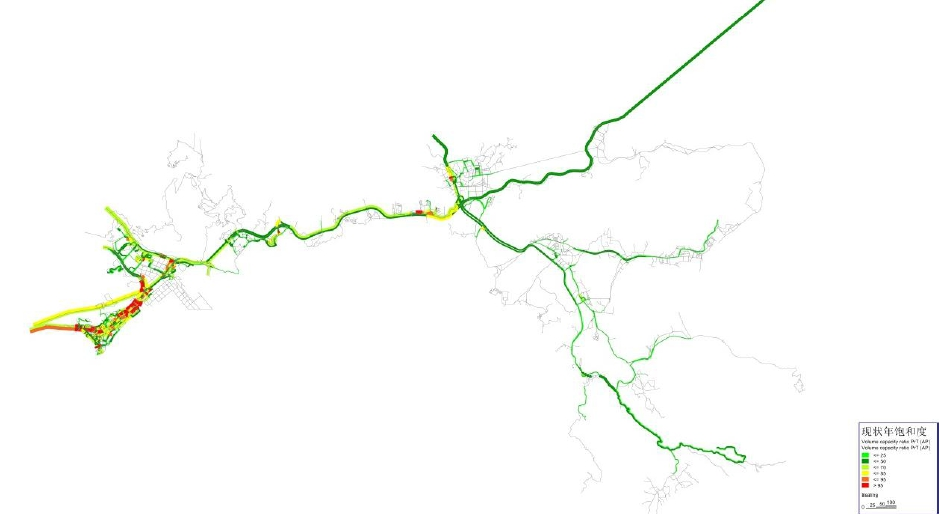
\includegraphics[width=\textwidth]{chp05_现状年盐田大鹏路段饱和度分布图.jpg}
  \caption{现状年盐田、大鹏路段饱和度分布图\label{fig:chp05_现状年盐田大鹏路段饱和度分布图} }
\end{figure}

\begin{figure}[!ht]
  \centering
  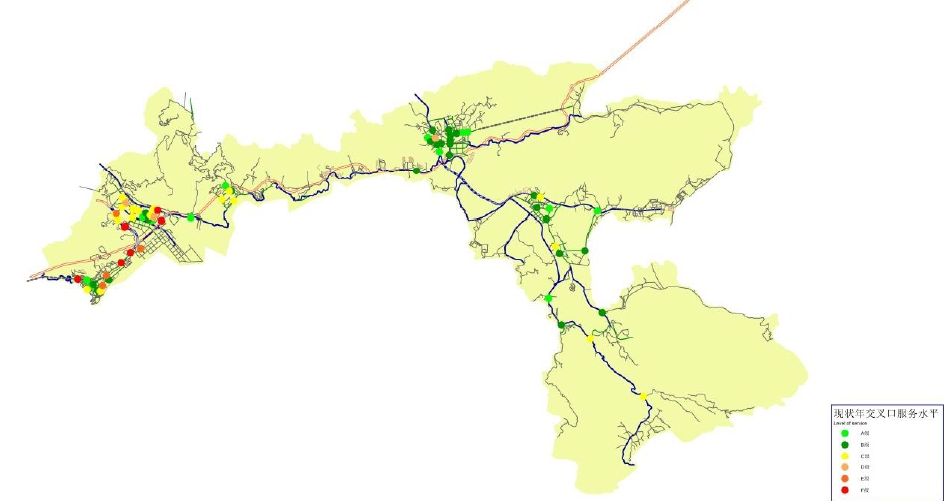
\includegraphics[width=\textwidth]{chp05_现状年盐田大鹏交叉口服务水平分布图.jpg}
  \caption{现状年盐田、大鹏交叉口服务水平分布图\label{fig:chp05_现状年盐田大鹏交叉口服务水平分布图} }
\end{figure}

\begin{figure}[!ht]
  \centering
  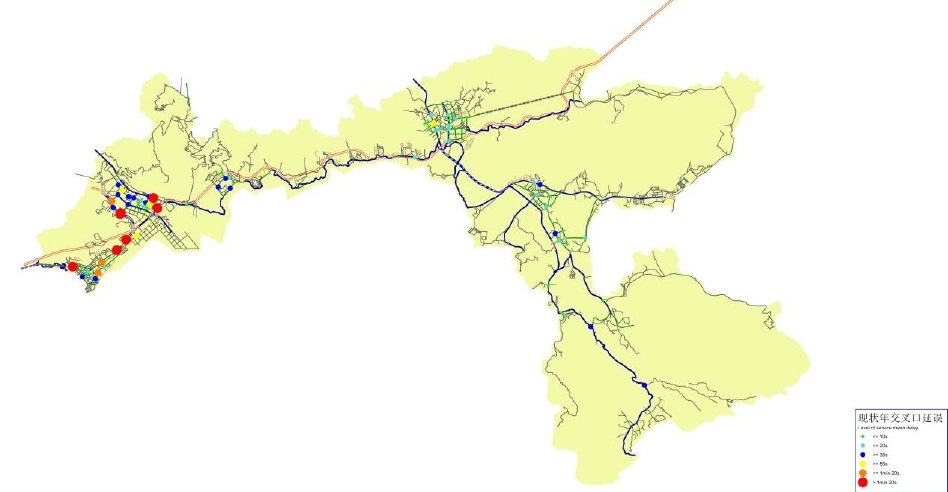
\includegraphics[width=\textwidth]{chp05_现状年盐田大鹏交叉口延误分布图.jpg}
  \caption{现状年盐田、大鹏交叉口延误分布图\label{fig:chp05_现状年盐田大鹏交叉口延误分布图} }
\end{figure}

\makeatletter
\setlength{\@fptop}{0pt}
\makeatother













